\documentclass{beamer}

\usetheme[subsectionpage=progressbar]{metropolis}
\setbeamertemplate{section in toc}[sections numbered]
\setbeamertemplate{subsection in toc}[subsections numbered]

\setbeamertemplate{frame numbering}[fraction]
% \useoutertheme{miniframes}
% \useinnertheme{rounded}
% \usefonttheme{metropolis}
\usecolortheme{spruce}
% \setbeamercolor{background canvas}{bg=white}
% \usecolortheme{wolverine}

\makeatletter
\setbeamertemplate{section page}{
  \centering
  \begin{minipage}{22em}
    \raggedright
    \usebeamercolor[fg]{section title}
    \usebeamerfont{section title}
    \thesection.~\insertsectionhead\\[-1ex]
    \usebeamertemplate*{progress bar in section page}
    \par
    \ifx\insertsubsectionhead\@empty\else%
      \usebeamercolor[fg]{subsection title}%
      \usebeamerfont{subsection title}%
      \thesection.\thesubsection~\insertsubsectionhead
      \fi
  \end{minipage}
  \par
  \vspace{\baselineskip}
}
\makeatother

% \hypersetup{pdfstartview={Fit}} % fits the presentation to the window when first displayed

\titlegraphic{\hfill
\includegraphics[width=.4\textwidth]{img/logo.png}}
\title{Longest Common Subsequences}
\subtitle{Seminar 2}
\author{\large Joris LIMONIER \hfill \textit{\tiny{Supervised by} \scriptsize George KERCHEV}}
% \institute{University of Luxembourg}
\date{May 31, 2021}



\begin{document}
\metroset{block=fill}

\maketitle

\begin{frame}{Table of Contents}
  \tableofcontents
\end{frame}


\section{Introduction}
\subsection{What are LCS ?}
\begin{frame}{What are LCS ?}
  \begin{block}{Notation}
    ``LCS" = Longest Common Subsequence(s)
  \end{block}
  \uncover<2->{
    \textbf{Example 1}
    \begin{center}
      \begin{tabular}{rccccccccccc}
        \uncover<1->{
        $S_1$ : &
                & \only<1-3>{A}\only<4->{\textcolor{magenta}{\textbf A}}
                & \only<1-4>{B}\only<5->{\textcolor{magenta}{\textbf B}}
                & \only<1-5>{A}\only<6->{\textcolor{magenta}{\textbf A}}
                & \only<1-6>{B}\only<7->{\textcolor{magenta}{\textbf B}}
                & B
        }                                                                 \\
        \uncover<3->{
        $S_2$ : &
                & \only<1-3>{A}\only<4->{\textcolor{magenta}{\textbf A}}
                & A
                & \only<1-4>{B}\only<5->{\textcolor{magenta}{\textbf B}}
                & \only<1-5>{A}\only<6->{\textcolor{magenta}{\textbf A}}
                & \only<1-6>{B}\only<7->{\textcolor{magenta}{\textbf B}}}
      \end{tabular}
    \end{center}
    \uncover<8->{
      \(\implies\) The LCS between $S_1$ and $S_2$ is \, \textcolor{magenta}{\textbf{A B A B}}
    }

    \uncover<9->{
      \vspace{.8cm}
      \textit{NB: LCS may not be unique, \,\textcolor{magenta}{A A B B}\, also works.}
    }
  }
\end{frame}

\begin{frame}[t]
  \textbf{Example 2}\\
  What is the LCS of the following sequences ?
  \begin{center}
    \begin{tabular}{rccccccccccc}
      \only<2>{
        $S_3$ :
       & AABBAABAAABABAAABAAABBABAAABAAABAAA \\
       & AAAABBABBBBAAABABBAABBAABBBBBAAAABA \\
       & BBABAAAABABAABBBABABBBBBAAABBBAABBB \\
       & AABAABBABABAABABBBBBBAABBBBBBAAAAAB \\
       & AABAAAAABAABAABAAABBABBBBABBAAAABBB \\
      }                                      \\
      \only<2>{
        $S_4$ :
       & BABBBABAABAABBBABBABBBBBBBABABAAABB \\
       & BBABBABBABBBABBBABBABBABABABBAABABA \\
       & BAABABAAAABABBABABBAAAABABBAABABABB \\
       & BABBBBBBAABAAABBABBBBAAAAABBBBBAAAB \\
       & ABBAAAABBBABABAABBABBBAABABBBABAABA \\
      }
    \end{tabular}
    \only<3>{
      
\includegraphics[width=.9\textwidth]{img/computing_the_lcs.jpg}
    }
  \end{center}
\end{frame}

\subsection{Why are we interested in LCS ?}

\begin{frame}[standout]
  Applications
\end{frame}

\begin{frame}[t]
  Applications:
    \begin{itemize}
      \item Bioinformatics: Compare sequences of nucleotides (DNA)
      \uncover<2->{\item Natural Language Processing: Compare texts}
      \uncover<3->{\item Computer Science: Spot differences in texts}
    \end{itemize}
    % \vfill
    \begin{center}
      \only<1>{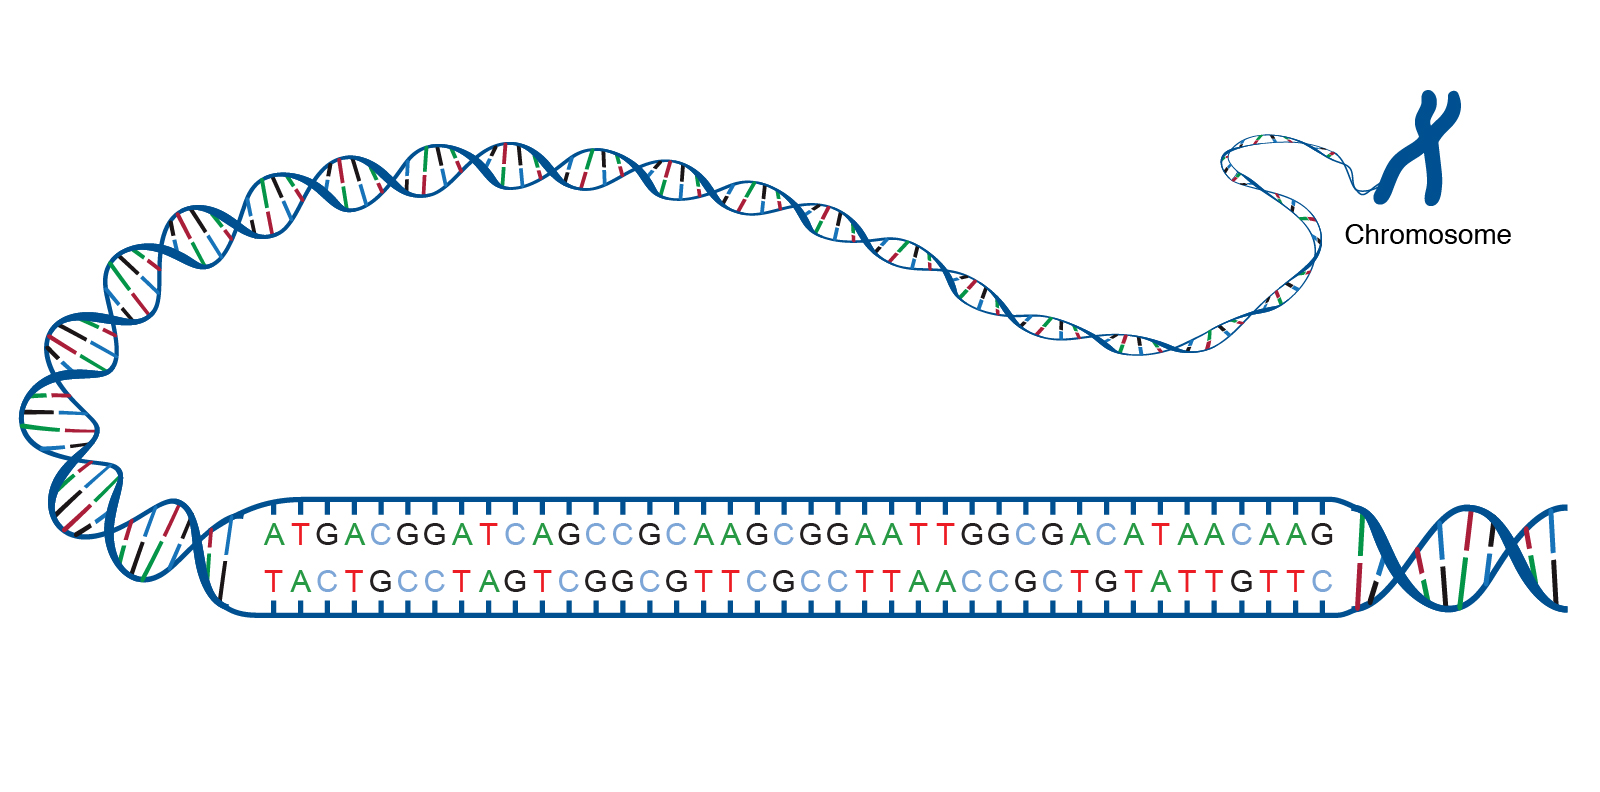
\includegraphics[width=.85\textwidth]{img/dna.jpg}}
      \only<2>{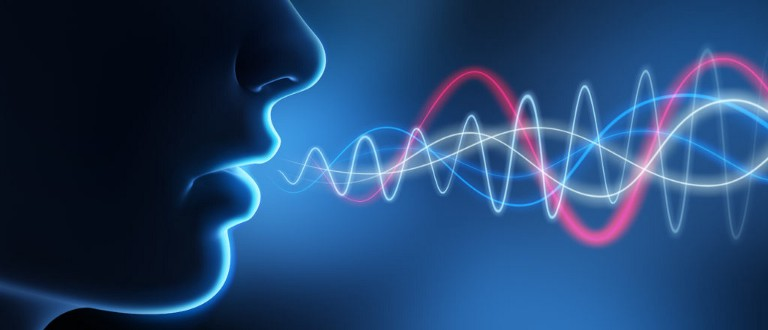
\includegraphics[width=1\textwidth]{img/nlp.jpeg}}
      \onslide<3>{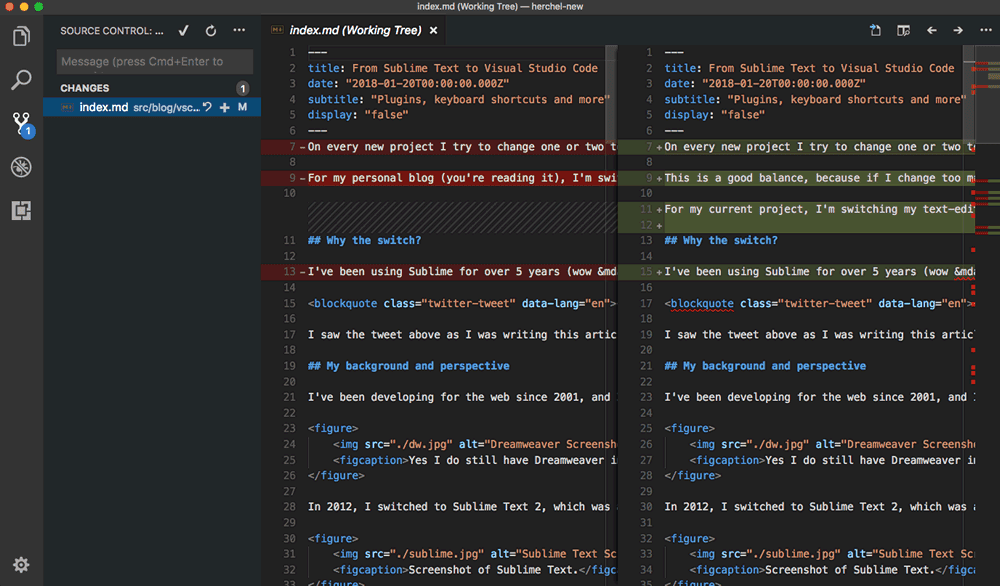
\includegraphics[width=.9\textwidth]{img/file_comparison.png}}
    \end{center}
\end{frame}

\section{How to find LCS ?}
\subsection{Step 1: Building the table}
\begin{frame}
\end{frame}

\subsection{Step 2: Crawling back up the table}
\begin{frame}
\end{frame}

\section{Data analysis of LCS results}
\subsection{Subsection 1}

\begin{frame}
\end{frame}

\begin{frame}[standout]
  Thank you
\end{frame}

\end{document}